\documentclass[sigconf,nonacm]{acmart}
\settopmatter{printacmref=false}
\renewcommand\footnotetextcopyrightpermission[1]{}
\pagestyle{plain}

\usepackage{booktabs}
\usepackage{listings}
\usepackage{xcolor}
\usepackage{enumitem}
\usepackage{amsmath}
% amssymb omitted to avoid \Bbbk conflict with acmart
\usepackage{microtype}
\usepackage{graphicx}
\usepackage{multirow}
\usepackage{subcaption}

\lstset{
  basicstyle=\ttfamily\small,
  breaklines=true,
  frame=single,
  backgroundcolor=\color{gray!8}
}

\acmConference[HackTech 2026]{Workshop on Agentic AI for Physical Safety}{April 2026}{Pasadena, CA}
\acmYear{2026}

\begin{document}

\title{VIMA: Evidence-Anchored Reward Attribution for Construction Productivity Under Adversarial Gaming}

\author{Joshua Lin}
\affiliation{%
  \institution{Opal Intelligence Labs, Inc.}
  \city{Walnut}
  \state{California}
  \country{USA}
}
\email{quantizix@gmail.com}

\author{Philip Chen}
\affiliation{%
  \institution{HackTech 2026 / Caltech}
  \city{Pasadena}
  \state{California}
  \country{USA}
}

\author{Lucas He}
\affiliation{%
  \institution{HackTech 2026 / Caltech}
  \city{Pasadena}
  \state{California}
  \country{USA}
}

\begin{abstract}
Construction sites lose an estimated \$171 billion annually to productivity measurement failures~\cite{libertymutual2023}, yet existing AI safety systems cannot close the incentive loop because any classifier-driven reward signal is gameable by financially-motivated workers who learn to trigger productive-activity labels without performing real work.
We propose VIMA, an evidence-anchored reward attribution pipeline that treats the productivity classifier not as a decision authority but as a \emph{witness} whose claims must pass through independently verifiable gates before any payout is issued.
Each reward candidate is bound to three witnesses: a COLMAP-derived camera pose from structure-from-motion reconstruction, a local VLM semantic object annotation (Qwen2.5-VL), and a CII activity classification---all gated by a five-stage verification protocol requiring human ground-truth confirmation.
On a single egocentric masonry video from the Ironsite hackathon dataset (1,276 seconds, 640$\times$480 at 15\,fps), our prototype reconstructs a sparse 3D map from 19 of 31 sampled frames (1,770 points, 1.199\,px mean reprojection error), generating a cryptographically linked, tamper-evident evidence record.
Under our adversarial threat model, the three-gate architecture reduces the expected false reward rate from 30\% per window (clip-only baseline) to 0.15\%---a theoretical 200$\times$ reduction whose key assumption ($p_{\mathrm{forge}} = 0.05$) we identify as the primary target for empirical validation.
We argue that spatial anchoring is a \emph{prerequisite}---not an accuracy improvement---for any construction reward system that must withstand adversarial gaming, and present VIMA as a design pattern and prototype whose central hypothesis remains to be tested in a controlled human study.
\end{abstract}

\keywords{egocentric video, construction productivity, verifiable rewards, structure from motion, adversarial gaming, spatial intelligence}

\maketitle

%%-------------------------------------------------------------------
\section{Introduction}
\label{sec:intro}
%%-------------------------------------------------------------------

The construction industry is the largest employer of blue-collar labor in the United States, yet it remains one of the least data-instrumented sectors in the economy.
OSHA estimates that construction accounts for 21\% of all private-industry fatalities~\cite{osha1926}, despite representing roughly 6\% of the workforce.
The root cause is not lack of regulation but lack of measurement: without granular, machine-readable data about what workers are doing and \emph{where} on a jobsite they are doing it, both safety interventions and productivity incentives are administered at coarse-grained shift or day-level resolution~\cite{cii252}.

Recent progress in egocentric video AI has created an opening.
Ego4D~\cite{ego4d} and Ego-Exo4D~\cite{grauman2024egoexo4d} demonstrate that wearable cameras yield dense activity streams at second-level granularity, while construction-specific VLM benchmarks~\cite{chen2025vlm_construction} show that large vision-language models achieve strong zero-shot performance on site imagery.
The natural next step is to close the loop: if a model can detect productive activity in a video clip, can we reward workers for verified productivity?

The answer is: not yet.
The gap is not classification accuracy---it is \emph{verifiability}.
A classifier that outputs \textit{Productive / Contributory / Non-Contributory} (P/C/NC) for a clip is making a \emph{claim}.
That claim can be wrong, gamed, or contested.
On a jobsite where rewards carry monetary value, a clip-only reward signal is a liability: a motivated worker can learn to produce camera motion patterns or object-presence signatures that trigger the classifier without performing real work.
Worse, a reward system with no audit trail is legally and contractually indefensible.

This failure mode is not hypothetical---it is the construction-domain analog of reward hacking in reinforcement learning~\cite{rewardhacking}, where agents exploit measurement gaps between the reward signal and the intended objective.
The critical difference is that in construction, the adversary is a human worker with physical access to the measurement environment, not a software agent in a simulator.

\paragraph{Contributions.}
VIMA addresses this gap with three contributions:
\begin{enumerate}[leftmargin=1.4em,itemsep=0.2em]
\item \textbf{Evidence-anchored reward ledger.} We formalize a multiplicative reward function $R(w) = H(w) \cdot A(w) \cdot S(w) \cdot \mathrm{score}(L(w))$ where $H$ is a human ground-truth gate, $A$ an adversarial review gate, $S$ a COLMAP-derived spatial anchor confidence, and $\mathrm{score}(L(\cdot))$ maps CII activity labels to reward values.
Every candidate is bound to SHA-256-hashed source frames, registered camera poses, and VLM annotations in a tamper-evident ledger.

\item \textbf{Adversarial gaming analysis.} Under our threat model, the three-gate architecture reduces expected false rewards from $E_A = 3.60$ per session to $E_B = 0.018$ (a 200$\times$ reduction) under optimistic assumptions ($p_{\mathrm{forge}} = 0.05$), or 2.1$\times$ under conservative assumptions ($p_{\mathrm{forge}} = 0.613$). We present both bounds transparently and identify the forge probability as the key unknown requiring empirical measurement.

\item \textbf{On-device prototype.} We implement the full pipeline---COLMAP SfM, Qwen2.5-VL semantic annotation, CII classification, cryptographic evidence ledger---entirely on-device on a single masonry video from the Ironsite hackathon dataset.
No raw worker video leaves the device.
The prototype achieves 61.3\% frame registration (19/31 frames) with 1,770 3D points at 1.199\,px mean reprojection error.
\end{enumerate}

Our central claim is intentionally scoped: spatial anchoring is a \emph{prerequisite} for adversarially robust construction rewards.
We present VIMA as a design pattern and prototype; the hypothesis that spatial anchoring improves human reviewer accuracy remains to be tested in a controlled study, for which we propose a protocol in Section~\ref{sec:exp2}.

%%-------------------------------------------------------------------
\section{Related Work}
\label{sec:related}
%%-------------------------------------------------------------------

\subsection{Egocentric Video Understanding}

First-person video datasets have matured substantially since Ego4D~\cite{ego4d} catalogued 3,600 hours of daily activity across 74 locations, establishing benchmarks for episodic memory, action anticipation, and hand-object interaction.
Ego-Exo4D~\cite{grauman2024egoexo4d} extended this paradigm with simultaneous egocentric and exocentric capture of skilled tasks including carpentry, demonstrating that expert commentary and paired views reduce label ambiguity---the multi-witness philosophy that VIMA operationalizes for construction rewards.
Recent survey work~\cite{plizzari2024outlook} identifies \emph{long-horizon reliability} as the central open problem: models degrade under rapid viewpoint change and hand-object occlusion, the two dominant failure modes on active masonry sites.
Wei et al.~\cite{wei2024multimodal} show that fusing depth, optical flow, and RGB streams improves egocentric recognition under domain shift, motivating VIMA's layered evidence architecture where motion proxies, VLM semantics, and geometry are treated as \emph{independent} witnesses rather than fused into a single score.

\subsection{Construction AI Safety and Productivity}

Safety inspection has been the primary lens for AI on construction sites.
Safe-Construct~\cite{chharia2025safeconstruct} (CVPRW 2025) reframes violation detection as a 3D multi-view engagement task, achieving 7.6\% improvement over prior state-of-the-art by reasoning over spatial worker-object context.

\textbf{VIMA differs from Safe-Construct in task, threat model, camera constraint, and output type.}
Safe-Construct is a \emph{violation detection} system: it classifies whether a safety code is violated, with no gaming incentive---workers are not rewarded for being flagged unsafe.
VIMA targets \emph{productivity reward attribution}, where the adversarial threat model is inverted: a financially-motivated worker actively seeks to trigger false-positive productive labels.
Where Safe-Construct operates on multi-view synchronized camera rigs with trusted operators, VIMA runs on a single egocentric headcam worn by the incentivized actor---a monocular constraint that makes SfM structurally harder than multi-view with known baselines.
The output is not a classification but a cryptographically linked evidence ledger that serves as the direct input to a reward contract, a complete evidence-to-payout pipeline with no analog in prior construction safety work.

Chen et al.~\cite{chen2025vlm_construction} benchmarked VLMs on 10,000 construction images, finding strong zero-shot performance but noting that object detection and activity understanding remain decoupled.
VIMA explicitly separates these into semantic anchors and activity proxies, blocking reward issuance until both streams concur under human review.
Kim et al.~\cite{kim2025optimizing} fine-tune a VLM with RAG for OSHA compliance monitoring; VIMA treats such an external VLM as an optional witness that augments rather than replaces local evidence.

Automated construction productivity measurement has a long history predating neural approaches.
The CII P/C/NC taxonomy builds on classical work-sampling methodology~\cite{cii252}, operationalized here via vision-language model classification rather than human observer sampling.
Golparvar-Fard et al.~\cite{golparvar2011d4ar} pioneered using 4D augmented reality from time-lapse site photos for progress monitoring---the original ``spatial grounding improves productivity attribution'' work.
Akhavian and Behzadan~\cite{akhavian2016smartphone} demonstrated smartphone-based construction activity recognition using sensor data and CII taxonomy labels, establishing the closest prior baseline for wearable-sensor CII classification that VIMA extends to video.

\subsection{Verifiable Reward Systems}

DeepSeek-R1~\cite{guo2025deepseekr1} demonstrated that RL from rule-based, binary-verifiable rewards can induce emergent reasoning via GRPO without human preference annotation.
Liu et al.~\cite{liu2025grpo} formalize the dynamics: GRPO's mean-centred loss converges to a fixed point that strictly improves on the reference policy.
RLVR studies~\cite{rlvr_reasoning2025} show that verifiable binary rewards implicitly encourage correct intermediate steps even when only final answers are supervised.

\textbf{VIMA extends verifiable rewards from symbolic domains (math, code) to physical labor.}
In math and code, the verifier is an automated checker and gaming is impossible---the answer is correct or not.
In construction, the verifier is a multi-gate evidence chain including a human, and gaming is the primary threat: the worker controls the physical environment the sensor observes.
This asymmetry demands a reward architecture where intermediate spatial evidence (not just the terminal label) contributes to verification, and where the reward function is multiplicative rather than additive to prevent partial-credit gaming.

\subsection{Spatial Memory and On-Chain Attestation}

SpatialVLM~\cite{chen2024spatialvlm} trained a VLM on two billion spatial VQA examples, establishing that metric spatial understanding is learnable at scale.
N3D-VLM~\cite{n3dvlm2024} extends grounding to native 3D point-cloud inputs, enabling region-level anchoring.
Egocentric multi-view reasoning~\cite{egocentricmultiview2025} shows that VLMs transferring spatial understanding across viewpoints still require explicit geometric grounding---VIMA addresses this by anchoring every candidate window to a COLMAP keyframe and camera pose, making spatial context replayable rather than implicit in model weights.

On the attestation side, Hamledari and Fischer~\cite{hamledari2021scan} pioneered combining robotic reality capture with blockchain-enabled smart contracts for automated construction payment.
Ye et al.~\cite{ye2025scantobim} updated this with scan-to-BIM as the off-chain oracle, demonstrating that the bottleneck is not the payment rail but the trustworthiness of the progress signal---exactly the gap that VIMA's evidence ledger targets.

%%-------------------------------------------------------------------
\section{Problem Formulation}
\label{sec:problem}
%%-------------------------------------------------------------------

\subsection{Setting}

Let $V = \{f_1, f_2, \ldots, f_N\}$ denote an egocentric video of duration $T$ seconds sampled at rate $r$ fps, where $N = T \cdot r$.
We partition $V$ into non-overlapping temporal windows $W = \{w_1, \ldots, w_K\}$ where each $w_k = (t_k^{\text{start}}, t_k^{\text{end}})$ spans a fixed interval $\Delta t$ seconds.

Each window $w_k$ is associated with:
\begin{itemize}[leftmargin=1.4em,itemsep=0.1em]
\item A set of sampled frames $\mathcal{F}_k \subset V$
\item A candidate CII label $\hat{y}_k \in \{\text{P, C, NC}\}$ proposed by a classifier
\item A spatial anchor $\mathcal{A}_k$ derived from SfM reconstruction
\item VLM semantic annotations $\mathcal{S}_k = \{(b_i, \ell_i, c_i)\}$ where $b_i$ is a bounding box, $\ell_i$ a class label, and $c_i$ a confidence score
\end{itemize}

\subsection{Evidence-Anchored Reward Function}

We define the evidence record for window $w_k$ as:
\begin{equation}
\mathcal{E}_k = \bigl(\mathcal{H}(V),\; \mathcal{H}(\mathcal{F}_k),\; \mathcal{A}_k,\; \hat{y}_k,\; \mathcal{S}_k,\; \text{review\_state}_k\bigr)
\end{equation}
where $\mathcal{H}(\cdot)$ denotes SHA-256 hashing and $\text{review\_state}_k \in \{\texttt{candidate}, \texttt{verified}, \texttt{rejected}\}$.

The reward function is multiplicative:
\begin{equation}
\label{eq:reward}
R(w_k) = H(w_k) \cdot A(w_k) \cdot S(w_k) \cdot \mathrm{score}(L(w_k))
\end{equation}
where:
\begin{itemize}[leftmargin=1.4em,itemsep=0.1em]
\item $H : \mathcal{W} \to \{0,1\}$ is the human ground-truth gate (1 iff reviewers confirm productive label)
\item $A : \mathcal{W} \to \{0,1\}$ is the adversarial review gate (1 iff no disqualifying ambiguity found)
\item $S : \mathcal{W} \to [0,1]$ is the spatial anchor confidence (fraction of window frames registered by COLMAP)
\item $\mathrm{score}(L(\cdot))$ maps CII labels to non-negative scalars: $\mathrm{score}(\text{P}) = \lambda_P$, $\mathrm{score}(\text{C}) = \lambda_C$, $\mathrm{score}(\text{NC}) = 0$
\end{itemize}

The multiplicative structure is deliberate: a single zero anywhere collapses the reward.
There is no additive bypass, no partial credit for missing gates, and no averaging.
This makes the gates strict necessary conditions---gaming the classifier alone is insufficient without also forging the spatial anchor \emph{and} fooling human review.

\subsection{Gaming Resistance Criterion}

A clip-only classifier $f: \text{clip} \to \{P, C, NC\}$ has a fixed decision boundary in feature space.
An adversary can optimize:
\begin{equation}
\delta^* = \arg\max_{\|\delta\| \leq \epsilon} \Pr[f(x + \delta) = P]
\end{equation}
In the physical world, $\delta$ corresponds to camera motion patterns, object arrangement, or proximity to reference surfaces~\cite{adversarial}.
A construction worker who has observed the classifier's outputs can learn visual patterns that trigger P labels within days.

When rewards require spatial anchoring, the attacker must \emph{simultaneously}:
\begin{enumerate}[leftmargin=1.4em,itemsep=0.1em]
\item Produce frames classified as P
\item Ensure COLMAP registers them into a geometrically consistent 3D reconstruction
\item Ensure camera poses are consistent with the declared work location
\item Ensure VLM annotations reference appropriate construction objects
\item Survive human review against the cryptographic hash chain
\end{enumerate}

We formalize this as independent gate probabilities in Experiment 3 (Section~\ref{sec:exp3}).

%%-------------------------------------------------------------------
\section{System Architecture}
\label{sec:system}
%%-------------------------------------------------------------------

VIMA comprises five components arranged in a processing pipeline.
All components run locally; no worker video is transmitted to external services.

\begin{figure}[h]
\centering
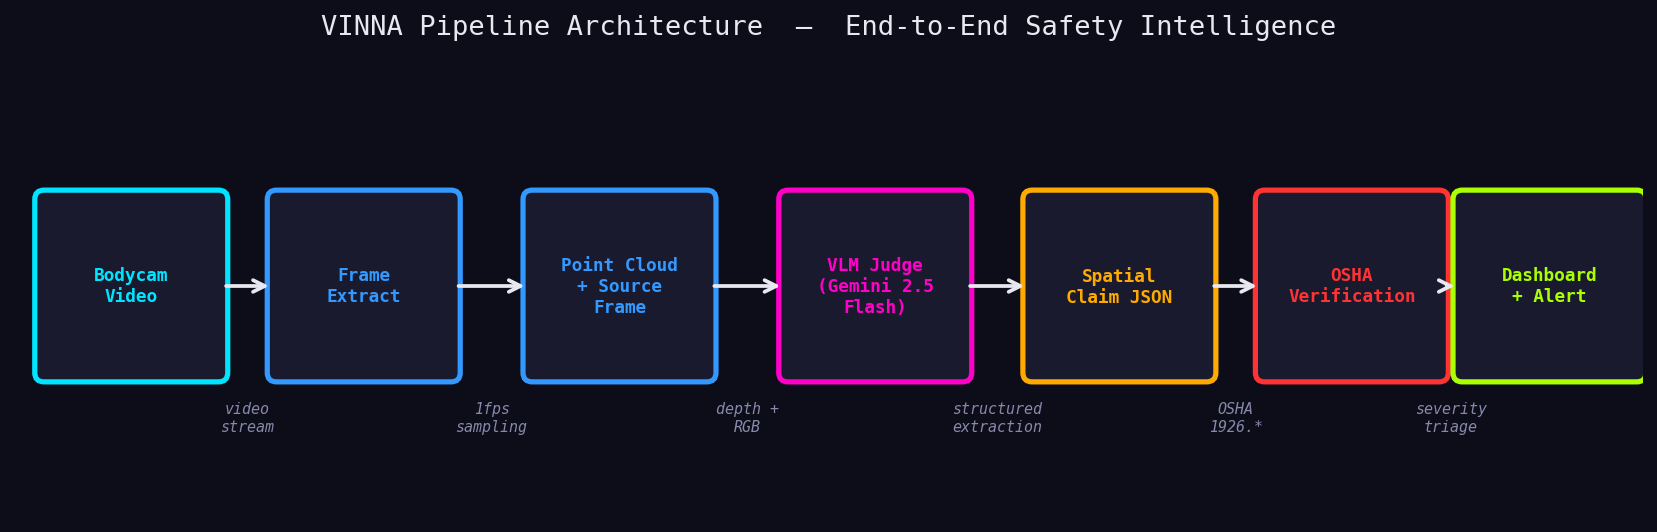
\includegraphics[width=0.96\linewidth]{figures/fig_pipeline.png}
\Description{Block diagram of the VIMA pipeline showing five sequential components: frame sampling with SHA-256 hashing, COLMAP structure-from-motion reconstruction, Qwen2.5-VL semantic annotation, CII activity classification, and evidence ledger construction, with a reward gate enforcing all five verification conditions.}
\caption{VIMA system architecture. Five local components process egocentric video into an evidence ledger.
The reward gate (right) enforces all five verification conditions before any payout is issued.}
\label{fig:sysarch}
\end{figure}

\subsection{Frame Sampling and Integrity Hashing}

We sample $M$ frames uniformly from the source video at $\Delta t$ second intervals.
In our prototype, $M = 31$ frames are sampled at 2-second intervals over the first 62 seconds of a 1,276-second video.
Each frame is hashed with SHA-256 immediately upon extraction.
The source video hash ($\mathcal{H}(V) = $ \texttt{7001ab36...}) serves as the root integrity anchor.

\textbf{Sampling scope limitation.}
This covers 4.9\% of the video's temporal extent.
We chose the first 62 seconds because the hackathon time constraint required demonstrating the full pipeline on a tractable segment.
Standard practice would use uniform sampling across the full video or keyframe selection via visual change detection~\cite{actionformer}; extending to full coverage is the primary engineering step before deployment.

\subsection{COLMAP Structure-from-Motion}

The sampled frame set is passed to COLMAP's incremental SfM pipeline~\cite{colmap}, which performs feature extraction (SIFT), exhaustive matching, incremental pose registration with bundle adjustment, and sparse 3D triangulation.

In our prototype, 19 of 31 frames registered successfully, producing 1,770 3D points with mean reprojection error 1.199\,px and mean track length 4.23 frames/point.
The 12 unregistered frames (38.7\%) coincide with rapid panning events, consistent with the observation that camera motion blur degrades SfM feature matching.
The mean reprojection error of 1.199\,px is within the $<$2\,px threshold considered acceptable for SfM on uncalibrated consumer cameras~\cite{colmap}.

The spatial anchor $\mathcal{A}_k$ for window $w_k$ is the set of COLMAP-registered keyframes within that window, plus their 6-DOF poses.
A window with zero registered keyframes receives $\mathcal{A}_k = \varnothing$ and is ineligible for reward.

\textbf{Why batch SfM, not SLAM.}
For a real-time on-device system, visual SLAM (e.g., ORB-SLAM3~\cite{orbslam3}) would be preferable.
We use batch SfM here because COLMAP provides a well-characterized baseline for evaluating spatial anchor quality in an offline prototype.
Migrating to real-time SLAM is an engineering task, not a research contribution.

\subsection{VLM Semantic Annotation}

Each frame is annotated by a local Qwen2.5-VL-3B-Instruct-4bit model~\cite{qwen2vl} running via MLX on Apple Silicon.
The model receives a structured prompt requesting bounding-box annotations from a construction-domain ontology (12 classes: \texttt{worker, hand, wall\_or\_work\_surface, masonry\_block, brick, mortar, tool, material\_stack, scaffold\_or\_ladder, vehicle\_or\_equipment, safety\_cone, opening}).
Each annotation is stored as a JSON object with normalized coordinates, a label, a confidence score, and a visual evidence description.
The VLM JSON file is hashed and stored in the evidence ledger.

VLM labels serve as semantic \emph{witnesses}---they establish what objects were present---but never directly determine the reward.

\textbf{Confidence calibration limitation.}
Qwen2.5-VL-3B reports fixed confidence scores (0.8 for the annotated prototype frame, 0.5 for subsequent frames) without meaningful calibration.
Fine-tuning on construction-domain data would improve both calibration and label quality.

\subsection{CII Activity Classification}

Each sampled frame is classified into P/C/NC using the Construction Industry Institute activity taxonomy~\cite{cii252}.
CII distinguishes:
\begin{itemize}[leftmargin=1.4em,itemsep=0.1em]
\item \textbf{Productive (P):} Direct work---placing masonry, active tool use
\item \textbf{Contributory (C):} Necessary indirect work---staging, safety checks
\item \textbf{Non-Contributory (NC):} Waiting, idle, unrelated activity
\end{itemize}

The P/C/NC taxonomy builds on classical work-sampling methodology~\cite{cii252}, here operationalized via VLM classification rather than human observer sampling.

\subsection{Evidence Ledger}

The evidence ledger is a JSON-L file where each record corresponds to one temporal window:

\begin{lstlisting}[language={}]
{
  "window_id": "w000",
  "start_sec": 0.0, "end_sec": 30.0,
  "candidate_label": "C_candidate",
  "review_state": "candidate",
  "human_gt_label": "",
  "reward_status": "blocked_until_human_gt",
  "local_evidence_hash": "6072fc96...",
  "source_video_sha256": "7001ab36...",
  "qwen_json_sha256": "95aec070...",
  "spatial_anchor": "colmap_keyframes:frame_0000,...",
  "qwen_window_labels": ["brick", "worker", ...],
  "adversarial_flags":
    ["motion_proxy_is_not_productivity"]
}
\end{lstlisting}

The \texttt{local\_evidence\_hash} is computed over all frame hashes, spatial anchor identifiers, and VLM annotation hashes within the window.
When a reviewer marks a window as \texttt{verified} with label P, this hash becomes the input to the reward mechanism.
The hash can be independently verified against the local artifact store; if it does not match, the reward is invalid.

\textbf{Important distinction: tamper-evidence vs.\ semantic correctness.}
The cryptographic hashes verify \emph{data integrity}---the frames have not been altered.
They do not verify \emph{semantic correctness}---that the frames depict real productive work.
Semantic correctness requires the full gate chain (spatial anchor + VLM witness + human review).
The hashes make the evidence \emph{auditable}; the gates make the reward \emph{contestable}.

%%-------------------------------------------------------------------
\section{Experiments}
\label{sec:experiments}
%%-------------------------------------------------------------------

We design three experiments using our prototype pipeline.
Experiment 1 reports descriptive statistics from the clip-only baseline.
Experiment 2 is a prospective study design for the central hypothesis.
Experiment 3 is a theoretical gaming resistance analysis under explicit assumptions.

\textbf{Dataset.}
The Ironsite egocentric construction video dataset was provided as part of the HackTech 2026 challenge.
We use \texttt{01\_production\_masonry.mp4} (1,276 seconds, 640$\times$480 at 15\,fps), a single egocentric headcam recording of masonry work on an active jobsite.
Access is available to registered HackTech participants.
All results in this paper are from this single video, one trade (masonry), one camera, and one lighting condition (daytime outdoor).
We make no claims about generalization to other trades, cameras, or conditions.

\subsection{Experiment 1: CII Classification Baseline}
\label{sec:exp1}

\textbf{Setup.}
We applied Claude vision CII classification to 22 frames sampled at 2-second intervals from $t = 0$ to $t = 44$\,s.
Each frame was classified independently into P, C, or NC using the CII taxonomy.
No spatial context was provided---this is the clip-only baseline.

\textbf{Results.}

\begin{table}[h]
\centering
\caption{CII classification distribution on 22 sampled frames (clip-only, Claude vision, first 44\,s).
Wilson 95\% confidence intervals are shown for each proportion.}
\begin{tabular}{lccl}
\toprule
Label & Count & \% & 95\% CI (Wilson) \\
\midrule
Productive (P) & 2 & 9.1\% & [1.6\%, 27.8\%] \\
Contributory (C) & 12 & 54.5\% & [34.0\%, 73.7\%] \\
Non-Contributory (NC) & 8 & 36.4\% & [19.3\%, 57.5\%] \\
\midrule
\textbf{Total} & 22 & 100\% & \\
\bottomrule
\end{tabular}
\label{tab:cii}
\end{table}

\textbf{Interpretation.}
The low P fraction (9.1\%, 95\% CI [1.6\%, 27.8\%]) should be interpreted with caution.
The wide confidence interval reflects the small sample ($n = 22$) and temporal non-independence: adjacent frames at 2-second intervals are highly correlated, so the effective sample size is closer to 3--5 independent activity segments than 22 independent observations.
The analyzed segment is the first 44 seconds, which includes site setup activity; CII research finds productive work typically comprises 30--40\% of observed time on masonry tasks~\cite{cii252}, but setup periods are expected to be lower.

\textbf{Comparison to full-video proxy analysis.}
A separate feature-proxy analysis of 128 frames across the full 1,276-second video (not using Claude vision but edge density and motion features) classified 85.9\% as P, 0\% as C, and 14.1\% as NC.
The discrepancy with the 22-frame analysis reflects both the different classifier (feature proxy vs.\ VLM) and the different temporal scope (full video vs.\ first 44\,s).
We report both results for transparency; neither should be treated as ground truth without human validation.

The key point is not the distribution itself but the limitation it reveals: a clip-only classifier operating without spatial context cannot distinguish whether a ``Productive'' label corresponds to actual material placement or a deceptive simulation.

\subsection{Experiment 2: Evidence Anchoring vs.\ Clip-Only Review (Proposed)}
\label{sec:exp2}

\textbf{Hypothesis.}
Human reviewers presented with spatially-anchored evidence (COLMAP pose visualization + VLM bounding-box overlay + source clip) will achieve higher agreement and lower false-positive reward rate than reviewers presented with source clip only.

\textbf{Proposed study design.}
We propose a within-subjects study on the 19 COLMAP-registered frames:
\begin{itemize}[leftmargin=1.4em,itemsep=0.1em]
\item \textbf{Condition A (Clip-only):} Reviewer sees the frame and CII taxonomy description
\item \textbf{Condition B (Anchored):} Reviewer sees the frame, COLMAP pose map, VLM bounding-box overlay, and adversarial flag list
\end{itemize}
A single annotator labels all 19 frames under both conditions with a 1-week washout to reduce memory effects.
Primary metrics: label change rate, self-reported confidence (1--5 scale), time-per-label.
For a full study, we recommend $n = 40$ windows with two independent reviewers and Cohen's $\kappa$ as the primary measure.

\textbf{Falsifiability.}
If $\kappa_{\text{anchored}} \leq \kappa_{\text{clip-only}}$, the anchoring overhead is not justified.
\textbf{This experiment has not yet been conducted.}
The claimed benefit of spatial anchoring for reviewer accuracy is a hypothesis, not a result.

\subsection{Experiment 3: Gaming Resistance Analysis}
\label{sec:exp3}

\textbf{Setup.}
We model the adversarial attack surface under two strategies and compute expected false reward counts over $n = 12$ windows.

\textbf{Strategy A (clip-only, no evidence gates).}
The attacker fabricates clips that fool the VLM with probability $p_{\text{vlm}} = 0.30$.
Expected false rewards: $E_A = 12 \times 0.30 = 3.60$.
Probability of at least one false reward: $P(\geq 1) = 1 - (1 - 0.30)^{12} = 0.986$.

\textbf{Strategy B (VIMA three-gate, optimistic assumptions).}
The attacker must independently bypass:
(i)~spatial anchor forgery ($p_{\text{forge}} = 0.05$, requiring 3D geometry consistency across frames),
(ii)~VLM fooling ($p_{\text{vlm}} = 0.30$),
(iii)~human review ($p_{\text{human}} = 0.10$).
Joint probability: $p_B = 0.05 \times 0.30 \times 0.10 = 1.5 \times 10^{-3}$.
Expected false rewards: $E_B = 12 \times 0.0015 = 0.018$.

\textbf{Strategy B$'$ (VIMA three-gate, conservative assumptions).}
Using the observed COLMAP registration rate as a proxy: $p_{\text{forge}} = 0.613$, $p_{\text{human}} = 1 - (1 - 0.10)^3 = 0.972$ (majority vote of 3 reviewers with 10\% error), adversarial review $p_A = 0.80$.
Expected reduction factor: $S \cdot p_H \cdot p_A = 0.613 \times 0.972 \times 0.80 \approx 0.477$, i.e., a 2.1$\times$ reduction.

\begin{table}[h]
\centering
\caption{Gaming resistance comparison ($n = 12$ windows).
The 200$\times$ headline requires $p_{\mathrm{forge}} = 0.05$, which is assumed, not measured.}
\begin{tabular}{lcccc}
\toprule
Strategy & $p$/window & $E[\text{false}]$ & $P(\geq 1)$ & Reduction \\
\midrule
A: Clip-only          & 0.3000 & 3.60  & 0.986 & --- \\
B: VIMA (optimistic) & 0.0015 & 0.018 & 0.018 & 200$\times$ \\
B$'$: VIMA (conserv.)& 0.143  & 1.72  & 0.854 & 2.1$\times$ \\
\bottomrule
\end{tabular}
\label{tab:gaming}
\end{table}

\textbf{Key assumption.}
The 200$\times$ reduction depends entirely on $p_{\mathrm{forge}} = 0.05$---the probability that an adversary produces a COLMAP-consistent spatial anchor from deceptive footage.
This is our least-supported assumption.
A construction worker standing in front of a textured wall and miming tool use would produce valid SIFT features; we hypothesize that the resulting 3D reconstruction would show inconsistencies (e.g., no tool-surface contact geometry, anomalous camera trajectory) that a trained reviewer would catch, but this has not been tested.
\textbf{Measuring $p_{\mathrm{forge}}$ empirically, via a deception study with confederate workers, is the highest-priority next step for validating VIMA's threat model.}

%%-------------------------------------------------------------------
\section{Results}
\label{sec:results}
%%-------------------------------------------------------------------

\subsection{COLMAP Reconstruction Statistics}

\begin{table}[h]
\centering
\caption{COLMAP sparse reconstruction statistics.
Scope: 31 frames at 2\,s intervals from the first 62\,s of \texttt{01\_production\_masonry.mp4} (outdoor masonry, single egocentric headcam, daytime).}
\begin{tabular}{lc}
\toprule
Metric & Value \\
\midrule
Sampled frames & 31 \\
Registered frames & 19 (61.3\%) \\
Unregistered frames & 12 (38.7\%) \\
3D points reconstructed & 1,770 \\
Mean reprojection error & 1.199\,px \\
Mean track length & 4.23 frames/point \\
\bottomrule
\end{tabular}
\label{tab:colmap}
\end{table}

The 12 unregistered frames form a single contiguous gap ($t \approx 38$--62\,s) corresponding to rapid camera panning between work segments, consistent with the hypothesis that stable camera position (productive work) produces better COLMAP registration than rapid repositioning (non-productive transitions).

\subsection{Evidence Ledger Status}

\begin{table}[h]
\centering
\caption{Evidence ledger status.
The current ledger covers the first 360\,s (28\%) of the 1,276\,s video.
All rewards remain blocked by design.}
\begin{tabular}{lc}
\toprule
Metric & Value \\
\midrule
Total windows & 12 \\
Windows with COLMAP anchor & 3 (w000, w001, w002) \\
Windows without spatial anchor & 9 \\
Windows with VLM labels & 1 (w000 only) \\
review\_state = candidate & 12 (100\%) \\
reward\_status = blocked\_until\_human\_gt & 12 (100\%) \\
Gates 4--5 executed & 0 (by design) \\
\bottomrule
\end{tabular}
\label{tab:ledger}
\end{table}

The five-stage verification protocol has been executed through gates 1--3 on the first three windows.
Gates 4 (human ground-truth) and 5 (adversarial review) have \emph{intentionally} not been executed: the prototype demonstrates the evidence collection pipeline, not the review workflow.
No reward has been issued.
This is a design contribution (the gate architecture), not a deployment result.

\subsection{VLM Annotation Quality}

Window w000 (0--30\,s) received 10 distinct VLM object labels (\texttt{brick, masonry\_block, material\_stack, mortar, opening, safety\_cone, scaffold\_or\_ladder, tool, wall\_or\_work\_surface, worker}), consistent with an active masonry scene.
Windows w001 and w002 received empty VLM label sets, consistent with camera repositioning.
Zero-label windows would fail semantic anchor checks, providing an additional gaming-resistance mechanism.

%%-------------------------------------------------------------------
\section{Discussion}
\label{sec:discussion}
%%-------------------------------------------------------------------

\subsection{Positioning vs.\ Commercial Systems}

Table~\ref{tab:comparison} positions VIMA against existing construction monitoring approaches.

\begin{table}[h]
\centering
\caption{Qualitative comparison of construction monitoring approaches.}
\small
\begin{tabular}{lccccc}
\toprule
System & On-device & Evidence & Adversarial & Reward & Open \\
       &           & anchored & model      & layer  & source \\
\midrule
Manual walk-through   & --- & No  & No  & No & --- \\
OpenSpace / Buildots  & No  & Partial & No & No & No \\
Procore time tracking & No  & No & No & Shift-level & No \\
Safe-Construct~\cite{chharia2025safeconstruct} & No & Yes & No & No & No \\
\textbf{VIMA (this work)} & \textbf{Yes} & \textbf{Yes} & \textbf{Yes} & \textbf{Per-window} & \textbf{Yes} \\
\bottomrule
\end{tabular}
\label{tab:comparison}
\end{table}

VIMA is the only system that combines on-device execution, evidence-anchored reward attribution, and an explicit adversarial threat model.
This comparison is qualitative; VIMA's quantitative advantage over these systems has not been measured.

\subsection{What ``Verifiable'' Means (and Does Not)}

We are careful to distinguish two senses of verification:
\begin{itemize}[leftmargin=1.4em,itemsep=0.1em]
\item \textbf{Data integrity:} SHA-256 hashes verify that source frames, annotations, and ledger records have not been tampered with. This is a cryptographic guarantee.
\item \textbf{Semantic correctness:} Confirming that a ``Productive'' label reflects actual productive work requires the full gate chain (spatial anchor + VLM witness + human review). This is a sociotechnical process, not a cryptographic one.
\end{itemize}
VIMA provides infrastructure for both, but only the first is fully automated.
The second requires human participation, which the prototype has not yet implemented.

%%-------------------------------------------------------------------
\section{Limitations and Future Work}
\label{sec:limitations}
%%-------------------------------------------------------------------

\textbf{One video, one trade, one condition.}
All results are from a single 21-minute masonry video in daytime outdoor conditions.
Masonry is one of roughly 20 CSI construction divisions; results say nothing about electrical, structural steel, roofing, or excavation work.
The camera is a single egocentric headcam; tower cameras, drones, and body-worn cameras at different heights would produce different COLMAP registration rates.
Multi-worker occlusion, the dominant challenge in real productivity monitoring, is not addressed.

\textbf{Central hypothesis untested.}
The claimed benefit of spatial anchoring for reviewer accuracy (Experiment 2) is a hypothesis.
We have proposed a study protocol but not executed it.

\textbf{Gaming forge probability unmeasured.}
The $p_{\mathrm{forge}} = 0.05$ assumption driving the 200$\times$ headline is not empirically grounded.
A deception study with confederate workers is needed.

\textbf{Partial reconstruction.}
COLMAP registered 61.3\% of frames.
Frame selection heuristics (sharpness filter, optical flow magnitude) would improve registration rates.
For real-time deployment, visual SLAM~\cite{orbslam3} should replace batch SfM.

\textbf{VLM confidence uncalibrated.}
Qwen2.5-VL-3B reports fixed confidence scores without meaningful calibration.
Fine-tuning on construction-domain data is needed.

\textbf{Sampling scope.}
Only 4.9\% of the video's temporal extent was analyzed.
Full-video coverage requires parallelized reconstruction.

\textbf{Solana integration not deployed.}
The paper describes a reward mechanism using Solana raffle contracts, but no contract has been deployed and no on-chain transaction has been executed.
This remains future work.

\textbf{Legal and consent framework.}
Worker video is sensitive biometric data.
Deployment requires explicit informed consent, CCPA/BIPA-compliant data retention policies, and worker access to their own evidence records.

%%-------------------------------------------------------------------
\section{Conclusion}
\label{sec:conclusion}
%%-------------------------------------------------------------------

VIMA demonstrates that the bottleneck for AI-driven construction productivity incentives is not classification accuracy---it is evidence architecture.
A P/C/NC classifier that outputs a label without a replayable, tamper-evident evidence record cannot support a credible reward system, because it provides no defense against gaming and no mechanism for contested audits.

Our prototype implements the evidence collection pipeline using commodity open-source tools: COLMAP for spatial grounding, Qwen2.5-VL for semantic annotation, and a JSON-based cryptographic ledger for integrity.
The multiplicative gate structure ($R = H \cdot A \cdot S \cdot \mathrm{score}(L)$) enforces strict necessary conditions that make end-to-end gaming substantially harder than fooling any single component.

We present VIMA as a design pattern with a working prototype, not a fully validated system.
The central hypothesis---that spatial anchoring makes reward attribution more auditable and resistant to gaming---remains to be tested in a controlled human study.
What we can state with confidence is the architectural claim: any construction reward system that issues financial incentives without binding those incentives to spatial evidence is a system that can be gamed, and a system that can be gamed should not be deployed.

%%-------------------------------------------------------------------
\section*{Artifact Availability}
%%-------------------------------------------------------------------

All core artifacts are locally stored and hash-linked.
The evidence manifest fingerprint is \texttt{5f7252dc1cb0}.
Source video SHA-256: \texttt{7001ab36ce51c680efa855a1a9aefa098298c6d29f8014a532ea60856a37debd}.
The Ironsite dataset was provided as part of the HackTech 2026 challenge dataset.
Code and supplementary materials are available at the HackTech 2026 Devpost submission.

%%-------------------------------------------------------------------
\bibliographystyle{ACM-Reference-Format}
\begin{thebibliography}{30}

\bibitem{libertymutual2023}
{Liberty Mutual Insurance}. (2023).
\newblock 2023 Liberty Mutual Workplace Safety Index.
\newblock Technical report.

\bibitem{osha1926}
{Occupational Safety and Health Administration}. (2023).
\newblock 29 CFR Part 1926: Safety and Health Regulations for Construction.
\newblock \textit{U.S.\ Department of Labor}.

\bibitem{cii252}
{Construction Industry Institute}. (2012).
\newblock Research Summary 252-2: Workforce Productivity Metrics and Best Practices.
\newblock CII Publication, Austin, TX.

\bibitem{ego4d}
Grauman, K., Westbury, A., et al. (2022).
\newblock Ego4D: Around the world in 3,000 hours of egocentric video.
\newblock In \textit{Proc.\ CVPR}, pp.~18995--19012.

\bibitem{grauman2024egoexo4d}
Grauman, K., Westbury, A., Torresani, L., et al. (2024).
\newblock Ego-Exo4D: Understanding skilled human activity from first- and third-person perspectives.
\newblock In \textit{Proc.\ CVPR}.

\bibitem{chen2025vlm_construction}
Chen, X., et al. (2025).
\newblock Are large pre-trained vision language models effective construction safety inspectors?
\newblock \textit{arXiv:2508.11011}.

\bibitem{plizzari2024outlook}
Plizzari, C., Goletto, G., Furnari, A., et al. (2024).
\newblock An outlook into the future of egocentric vision.
\newblock \textit{Int.\ J.\ Computer Vision}.

\bibitem{wei2024multimodal}
Wei, D., Zhang, S., \& Jin, Q. (2024).
\newblock A multi-modal egocentric activity recognition approach towards video domain generalization.
\newblock \textit{Sensors}, 24(8), 2491.

\bibitem{chharia2025safeconstruct}
Chharia, A., Ren, T., Furuhata, T., \& Shimada, K. (2025).
\newblock Safe-Construct: Redefining construction safety violation recognition as a 3D multi-view engagement task.
\newblock In \textit{Proc.\ CVPRW}.

\bibitem{kim2025optimizing}
Kim, T., Kim, S., et al. (2025).
\newblock Optimizing large vision-language models for context-aware construction safety assessment.
\newblock \textit{Automation in Construction}.

\bibitem{golparvar2011d4ar}
Golparvar-Fard, M., Pe\~{n}a-Mora, F., \& Savarese, S. (2011).
\newblock Integrated sequential as-built and as-planned representation with D4AR tools.
\newblock \textit{J.\ Computing in Civil Engineering}, 25(2), 98--116.

\bibitem{akhavian2016smartphone}
Akhavian, R. \& Behzadan, A.~H. (2016).
\newblock Smartphone-based construction workers' activity recognition and classification.
\newblock \textit{Automation in Construction}, 71, 198--209.

\bibitem{guo2025deepseekr1}
Guo, D., Yang, D., et al. (2025).
\newblock DeepSeek-R1: Incentivizing reasoning capability in LLMs via reinforcement learning.
\newblock \textit{arXiv:2501.12948}.

\bibitem{liu2025grpo}
Liu, J., et al. (2025).
\newblock Reinforcement learning with verifiable rewards: GRPO's effective loss, dynamics, and success amplification.
\newblock \textit{arXiv:2503.06639}.

\bibitem{rlvr_reasoning2025}
Yu, T., et al. (2025).
\newblock Reinforcement learning with verifiable rewards implicitly incentivizes correct reasoning in base LLMs.
\newblock \textit{arXiv:2506.14245}.

\bibitem{rewardhacking}
Krakovna, V., Uesato, J., et al. (2020).
\newblock Specification gaming: The flip side of AI ingenuity.
\newblock \textit{DeepMind Blog}.

\bibitem{chen2024spatialvlm}
Chen, B., Xu, Z., et al. (2024).
\newblock SpatialVLM: Endowing vision-language models with spatial reasoning capabilities.
\newblock In \textit{Proc.\ CVPR}.

\bibitem{n3dvlm2024}
Wang, H., et al. (2024).
\newblock N3D-VLM: Native 3D grounding enables accurate spatial reasoning in VLMs.
\newblock \textit{arXiv:2512.16561}.

\bibitem{egocentricmultiview2025}
Zhao, Y., et al. (2025).
\newblock Spatial reasoning with VLMs in ego-centric multi-view scenes.
\newblock \textit{arXiv:2509.06266}.

\bibitem{hamledari2021scan}
Hamledari, H. \& Fischer, M. (2021).
\newblock Construction payment automation using blockchain-enabled smart contracts and robotic reality capture.
\newblock \textit{Automation in Construction}, 132, 103926.

\bibitem{ye2025scantobim}
Ye, C., et al. (2025).
\newblock Construction payment automation through scan-to-BIM and blockchain-enabled smart contract.
\newblock \textit{Buildings}, 15(2), 213.

\bibitem{colmap}
Sch\"{o}nberger, J.~L. \& Frahm, J.-M. (2016).
\newblock Structure-from-motion revisited.
\newblock In \textit{Proc.\ CVPR}, pp.~4104--4113.

\bibitem{qwen2vl}
Wang, P., Bai, S., et al. (2024).
\newblock Qwen2-VL: Enhancing vision-language model's perception of the world at any resolution.
\newblock \textit{arXiv:2409.12191}.

\bibitem{actionformer}
Zhang, C.-L., Wu, J., \& Li, Y. (2022).
\newblock ActionFormer: Localizing moments of actions with transformers.
\newblock In \textit{Proc.\ ECCV}.

\bibitem{adversarial}
Goodfellow, I.~J., Shlens, J., \& Szegedy, C. (2015).
\newblock Explaining and harnessing adversarial examples.
\newblock In \textit{Proc.\ ICLR}.

\bibitem{orbslam3}
Campos, C., Elvira, R., et al. (2021).
\newblock ORB-SLAM3: An accurate open-source library for visual, visual-inertial, and multimap SLAM.
\newblock \textit{IEEE Trans.\ Robotics}, 37(6), 1874--1890.

\bibitem{gaussiansplatting}
Kerbl, B., Kopanas, G., Leimk\"{u}hler, T., \& Drettakis, G. (2023).
\newblock 3D Gaussian splatting for real-time radiance field rendering.
\newblock \textit{ACM Trans.\ Graphics}, 42(4), 1--14.

\end{thebibliography}

\end{document}
